\documentclass{article}
\usepackage{graphicx} % Required for inserting images
\usepackage{asymptote}
\usepackage{hyperref}

\title{A Strange Shape: Aperiodic Monotiles}
\author{William Gvozdjak}
\date{December 2023}

\begin{document}

\maketitle

Suppose we had a tiling. For example, we can tile the plane with squares as follows:

\begin{center}
    \begin{asy}
        unitsize(0.75cm);
        int sidelength = 3;
        for (int i = 0; i < sidelength+1; ++i) {
            draw((i, -0.5)--(i, sidelength+0.5));
            draw((-0.5, i)--(sidelength+0.5, i));
        }
    \end{asy}
\end{center}

Now, what if I told you that there exists one shape, so that if we tile the plane, it \textit{never} repeats?

Let me explain. First, we need to define what ``repeating'' really is, since it's a little vague given that we're working with tilings to infinity. Imagine we have the above tiling. It obviously repeats: if we shift the entire plane to the right by one unit, it'll look the exact same. Now, cut the middle square in half:

\begin{center}
    \begin{asy}
        unitsize(0.75cm);
        int sidelength = 3;
        for (int i = 0; i < sidelength+1; ++i) {
            draw((i, -0.5)--(i, sidelength+0.5));
            draw((-0.5, i)--(sidelength+0.5, i));
        }
        draw((1.5, 1)--(1.5, 2));
    \end{asy}
\end{center}

Technically, this doesn't ever repeat: no matter how much we translate the entire plane by, if it's a nonzero amount, we'll never get the exact same configuration. But this example is boring; cutting one of the rectangles is an uninteresting way to get an ``non-repeating tiling.'' So, we'll enhance our definition.

Instead of just saying that the \textit{whole} configuration can't repeat, we'll say that there can't be \textit{arbitrarily large} part of the configuration that repeats. What does this mean? We say that, yes, some finite part of the configuration may repeat. But we ban ourselves from finding larger and larger parts of the configuration that repeat. This rules out the configuration we had with a square cut, since there are arbitrarily large subsets of it that look exactly like that full square tiling--and those do repeat! We say that an \textit{aperiodic tiling} is one that doesn't repeat.

So, now that we know what an aperiodic tiling is, we can take a look at which ones exist. The most famous examples of aperiodic tilings are known as \textit{Penrose tilings}. There are three different types of Penrose tilings, known as P1, P2, and P3. Each one uses three different sets of shapes. For example, this is one Penrose tiling:

\begin{center}
    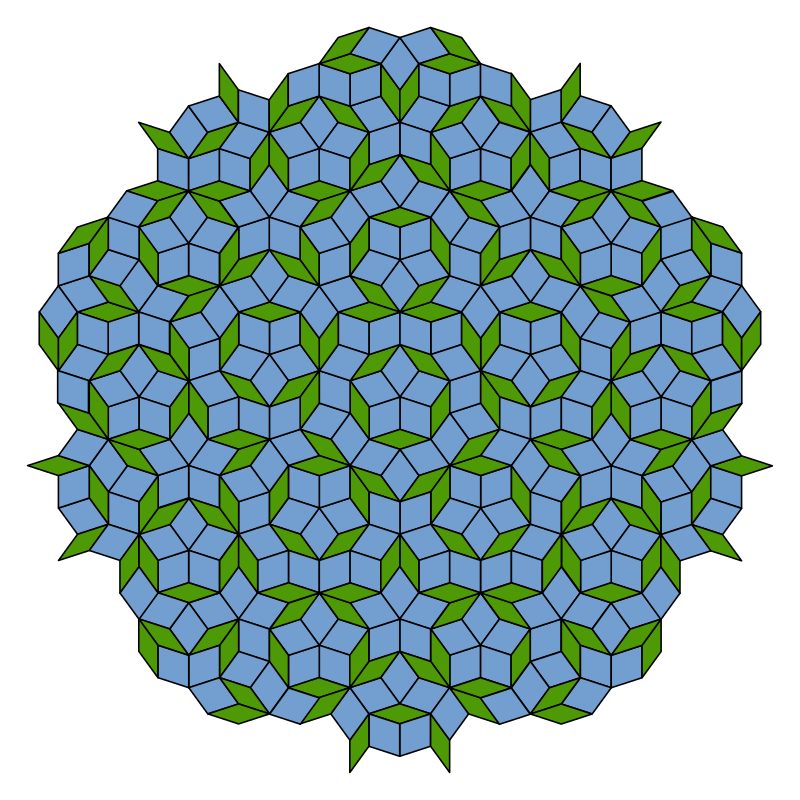
\includegraphics[width=2in]{images/penrose.png}
\end{center}

But there's one important thing that's in common between all the Penrose tilings: they all involve more than one shape. Specifically, both P1 has three different shapes, while both P2 and P3 have two different shapes. This led to the long-standing question: does there exist an aperiodic tiling that just uses \textit{one} shape? This question is often known as the \textbf{Einstein problem}.

Well, just this past year, an answer to this question was found by mathematicians Smith, Myers, Kaplan, and Goodman-Strauss: yes! How does the tiling look? The following is the shape used:

\begin{center}
    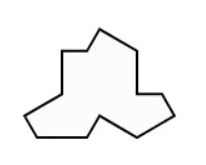
\includegraphics[width=1in]{images/einsteintile.png}
\end{center}

This shape is affectionately named the ``hat.'' The following is how it looks when we tile the whole plane:

\begin{center}
    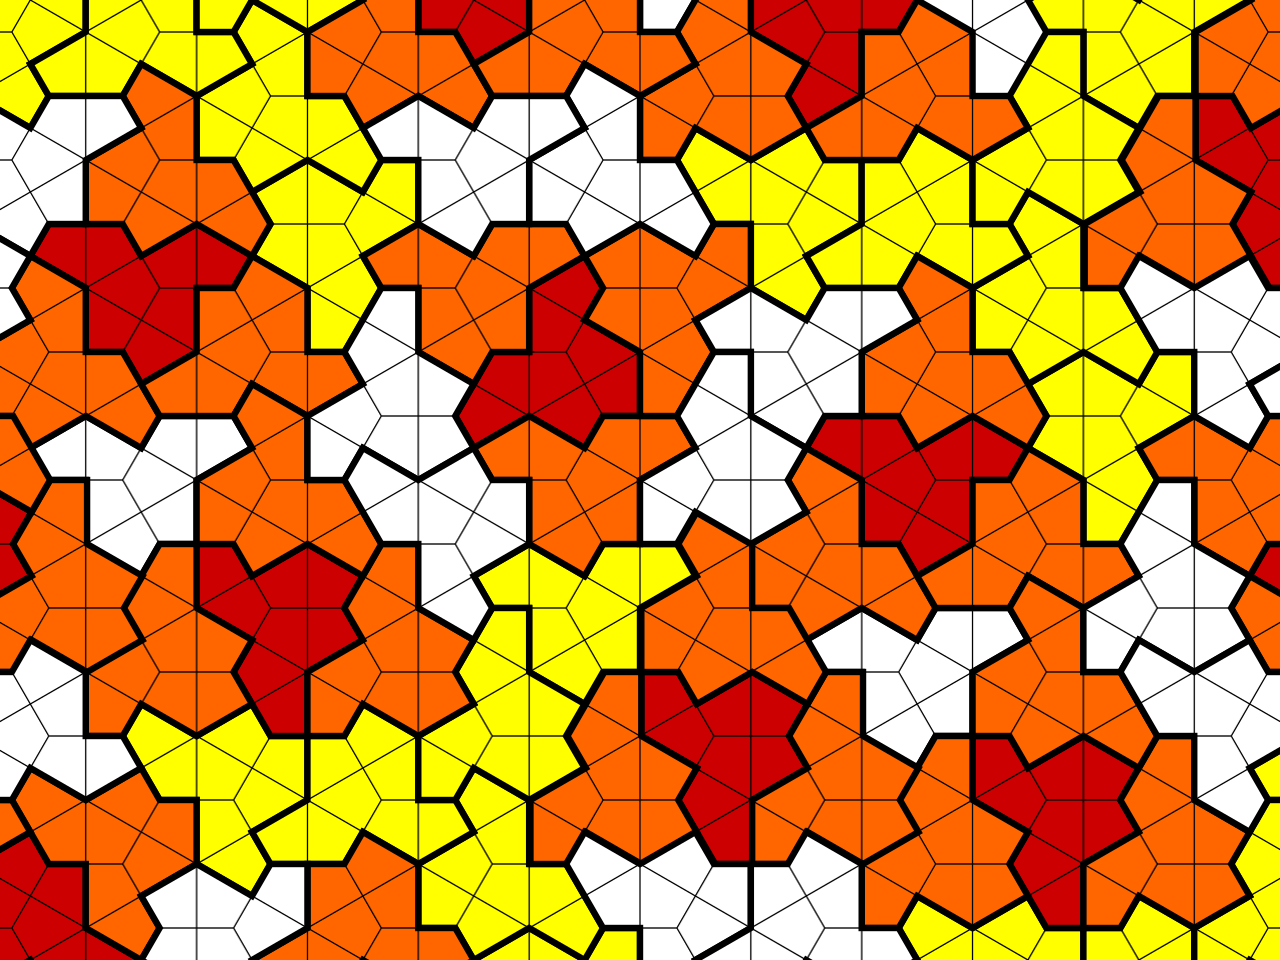
\includegraphics[width=2in]{images/einsteintiling.png}
\end{center}

But there was one concern raised: this tiling involves flipping the hat over and using that, so, technically, it isn't just that one tile--it also involves the reflected hat. Is there a tile that aperiodically tiles the plane without reflections? Once again, they answered this question: yes!

It turns out that this shape actually generalizes to an infinite family of tiles, all that tile the plane aperiodically by themselves. Among this family is a new shape, called the ``spectre tile,'' which aperiodically tiles the plane without reflections. Pretty cool!

All of the shapes in this family, along with any other tiles that potentially aperiodically tile the plane to infinity, are known as \textit{aperiodic monotiles}.

If you're interested in looking more into the aperiodic monotile that Smith, Myers, Kaplan, and Goodman-Strauss found, you can check out their paper on the arXiv preprint server at \url{https://arxiv.org/abs/2303.10798}.


\end{document}
